% Metódy inžinierskej práce
    \centering
    \label{fig:enter-label}
\documentclass[10pt,twocolumn,slovak,a4paper]{coursepaper}

\usepackage[slovak]{babel}
%\usepackage[T1]{fontenc}
\usepackage[IL2]{fontenc} % lepšia sadzba písmena Ľ než v T1
\usepackage[utf8]{inputenc}
\usepackage{graphicx}
\usepackage{wrapfig}
\usepackage{amsmath}
\usepackage{url} % príkaz \url na formátovanie URL
\usepackage{hyperref} % odkazy v texte budú aktívne (pri niektorých triedach dokumentov spôsobuje posun textu)

\usepackage{cite}
%\usepackage{times}

\pagestyle{headings}

\title{Hybrid music recommendations systems\thanks{Semestrálny projekt v predmete Metódy inžinierskej práce, ak. rok 2024/25, vedenie: Meno Priezvisko}} % meno a priezvisko vyučujúceho na cvičeniach

\author{Lukáš Orth\\[2pt]
	{\small Slovenská technická univerzita v Bratislave}\\
	{\small Fakulta informatiky a informačných technológií}\\
	{\small \texttt{xorth@stuba.sk}}
	}

\date{\small 30. september 2024} % upravte



\begin{document}

\maketitle

\begin{abstract}
Odporúčacie systémy zohrávajú kľúčovú rolu v zábavnom priemysle, najmä v moderných hudobných streamovacích platformách ako Spotify, Tidal, Deezer a iné. Ich úlohou je pomôcť užívateľom objaviť nové skladby, ktoré vyhovujú ich preferenciám. Bez nich by užívatelia mohli dostávať nežiadaný obsah, ktorý by pre nich mohol tvoriť zbytočne zlé skúsenosti. Konvenčné spôsoby riešia túto výzvu metódami, ktoré s	ú síce relatívne úspešné, ale prinášajú so sebou určité nevýhody a nedostatky. V oblasti streamovania hudby sa to prejavuje napríklad problémom studeného štartu. Tento problém v digitálnom priestore trápi najmä nových umelcov, o ktorých je málo známych informácií. Bez účinných odporúčacích mechanizmov môžu títo umelci čeliť ťažkostiam pri získavaní pozornosti a budovaní si fanúšikovskej základne. Zároveň môžu používatelia dostávať odporúčania, ktoré nezohľadňujú ich preferencie, čo vedie k frustrácii a negatívnym skúsenostiam s platformami.
\begin{wrapfigure}{r}{0.5\textwidth}
  \begin{center}
    
\includegraphics[width=0.2\textwidth]{STU-FIIT-nfh.png}
  \end{center}
  \caption{}
\end{wrapfigure}
V mojom článku sa budem podrobnejšie venovať tomuto problému, konkrétne prístupmi, ktoré by mohli zlepšiť skúsenosti používateľov a podporiť nové talenty. Hybridný systém odporúčania, ktorý kombinuje viaceré metódy, ako sú kolaboratívne odporúčanie a obsahové odporúčania, môže významne zvýšiť presnosť predpovedí. V článku vysvetlím, ako tento systém funguje, a predstavím experimenty, ktoré vykonali iní vedci. Následne sa pozriem na výsledky týchto experimentov a na záver zhrniem kľúčové zistenia. Cieľom mojej práce je zrozumiteľne spracovať tento problém a systém ktorý ho rieši, aby čitatelia pochopili, prečo je nevyhnutné inovovať odporúčacie systémy v hudobnom priemysle a aký prínos to môže mať pre objavovanie nových talentov.


\ldots
\end{abstract}


\begin{figure*}[h]
  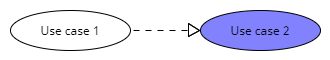
\includegraphics[width=\textwidth,height=4cm]{diagramtest1.png}
\end{figure*}



\begin{figure}[!tbp]
  \centering
  \begin{minipage}[b]{0.4\textwidth}
 \centering
    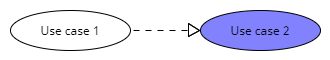
\includegraphics[width=1\textwidth]{diagramtest1.png}
    \caption{diagram 1}
  \end{minipage}
  \hfill
  \begin{minipage}[b]{0.4\textwidth}
 \centering
    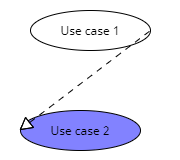
\includegraphics[width=0.5\textwidth]{diagramtest2.png}
    \caption{diagram 2}
  \end{minipage}
\end{figure}

\[
\begin{bmatrix}
1 & 2 & 3 & 4\\
a & b & c & d\\
1 & 2 & 3 & 4\\
a & b & c & d\\
1 & 2 & 3 & 4
\end{bmatrix}
\]

\section{Úvod}

Motivujte čitateľa a vysvetlite, o čom píšete. Úvod sa väčšinou nedelí na časti.

Uveďte explicitne štruktúru článku. Tu je nejaký príklad.
Základný problém, ktorý bol naznačený v úvode, je podrobnejšie vysvetlený v časti~\ref{nejaka}.
Dôležité súvislosti sú uvedené v častiach~\ref{dolezita} a~\ref{dolezitejsia}.
Záverečné poznámky prináša časť~\ref{zaver}.



\section{Nejaká časť} \label{nejaka}

Z obr.~\ref{f:rozhod} je všetko jasné. 

\begin{figure*}[tbh]
\centering
%\includegraphics[scale=1.0]{diagram.pdf}
Aj text môže byť prezentovaný ako obrázok. Stane sa z neho označný plávajúci objekt. Po vytvorení diagramu zrušte znak \texttt{\%} pred príkazom \verb|\includegraphics| označte tento riadok ako komentár (tiež pomocou znaku \texttt{\%}).
\caption{Rozhodujúci argument.}
\label{f:rozhod}
\end{figure*}



\section{Iná časť} \label{ina}

Základným problémom je teda\ldots{} Najprv sa pozrieme na nejaké vysvetlenie (časť~\ref{ina:nejake}), a potom na ešte nejaké (časť~\ref{ina:nejake}).\footnote{Niekedy môžete potrebovať aj poznámku pod čiarou.}

Môže sa zdať, že problém vlastne nejestvuje\cite{Coplien:MPD}, ale bolo dokázané, že to tak nie je~\cite{Czarnecki:Staged, Czarnecki:Progress}. Napriek tomu, aj dnes na webe narazíme na všelijaké pochybné názory\cite{PLP-Framework}. Dôležité veci možno \emph{zdôrazniť kurzívou}.


\subsection{Nejaké vysvetlenie} \label{ina:nejake}

Niekedy treba uviesť zoznam:

\begin{itemize}
\item jedna vec
\item druhá vec
	\begin{itemize}
	\item x
	\item y
	\end{itemize}
\end{itemize}

Ten istý zoznam, len číslovaný:

\begin{enumerate}
\item jedna vec
\item druhá vec
	\begin{enumerate}
	\item x
	\item y
	\end{enumerate}
\end{enumerate}


\subsection{Ešte nejaké vysvetlenie} \label{ina:este}

\paragraph{Veľmi dôležitá poznámka.}
Niekedy je potrebné nadpisom označiť odsek. Text pokračuje hneď za nadpisom.



\section{Dôležitá časť} \label{dolezita}




\section{Ešte dôležitejšia časť} \label{dolezitejsia}




\section{Záver} \label{zaver} % prípadne iný variant názvu



%\acknowledgement{Ak niekomu chcete poďakovať\ldots}


% týmto sa generuje zoznam literatúry z obsahu súboru literatura.bib podľa toho, na čo sa v článku odkazujete
\bibliography{literatura}
\bibliographystyle{plain} % prípadne alpha, abbrv alebo hociktorý iný
\end{document}
